\documentclass[conference]{IEEEtran}

\usepackage{cite}
\usepackage{amsmath,amssymb}
\usepackage{booktabs}
\usepackage{graphicx}
\usepackage{placeins}
\usepackage{float}
\usepackage{balance}
\usepackage{array}
\usepackage{url}

\graphicspath{{generated/}}
\DeclareGraphicsExtensions{.pdf,.png}
\setlength{\textfloatsep}{5pt plus 2pt minus 2pt}
\setlength{\dbltextfloatsep}{5pt plus 2pt minus 2pt}
\setlength{\floatsep}{4pt plus 1pt minus 1pt}
\setlength{\abovecaptionskip}{3pt}
\setlength{\belowcaptionskip}{0pt}

\title{AERIS: Boundary-Mapped Reliable Routing for Wireless Sensor Networks under Heterogeneous Channels}

\author{
\IEEEauthorblockN{Kangrui Li, Junyi Lin, and Xiaobo Zhang}
\IEEEauthorblockA{Faculty of Automation, Guangdong University of Technology, Guangzhou 510006, China\\
\textit{Corresponding author:} Kangrui Li \texttt{1403073295@mails.gdut.edu.cn}}
}

\begin{document}

\maketitle

\begin{abstract}
AERIS is a rule-based hierarchical routing protocol for wireless sensor networks under heterogeneous channels. We evaluate it with an audited NS-3 evidence chain, including a seven-protocol dual-machine sweep against LEACH, PEGASIS, HEED, TEEN, CTP, and RPL-MRHOF across four environments and 50--1000 nodes ($n=30$ per environment-node-protocol cell). The expanded audit changes the claim from a global ranking to a boundary map. Against the classical WSN baselines, AERIS is rank-1 in 21 of 28 environment-node cells and top-2 in all 28. After adding CTP and RPL-MRHOF, AERIS remains rank-1 mainly in outdoor suburban cells (6 of 7 scales, with a near tie at 1000 nodes), while CTP leads benign office cells and RPL-MRHOF leads most factory and urban cells. A new 3360-run NS-3 ablation and an audited 400-replicate mechanism study show that AERIS's gain is carried mainly by Gateway-assisted uplinks, while first-node death falls to 1--4.5 rounds in most harsh 500/1000-node cells. The result is a sharper deployment rule: AERIS is useful when simple, auditable WSN routing needs stronger delivery than classical baselines provide, but it is not a replacement for richer collection-tree or RPL-style stacks in all regimes.
\end{abstract}

\begin{IEEEkeywords}
wireless sensor networks, reliable routing, cross-platform evaluation, deployment boundary
\end{IEEEkeywords}

\section{Introduction}
Wireless sensor network (WSN) routing is usually discussed in terms of energy, yet in many deployments link stability matters just as much \cite{akyildiz2002survey,rault2014energy,kandris2009power}. This becomes clear when classical protocols are placed side by side: LEACH emphasizes clustered forwarding \cite{heinzelman2000energy}, PEGASIS uses chain-based aggregation \cite{lindsey2002pegasis}, HEED relies on residual-energy-aware head election \cite{younis2004heed}, and TEEN reports only when event thresholds are crossed \cite{manjeshwar2001teen}. Real links make the trade-off harder because low-power WSN channels are asymmetric, environment sensitive, and often unstable near connectivity thresholds \cite{zuniga2004analyzing,zamalloa2007analysis,baccour2012radio}.

This leads to a practical question: when do simple, auditable control rules improve on classical energy-first designs under harsh channels, and when are richer collection-tree or RPL-style stacks the better answer? AERIS addresses the first half of this question with fixed-rule control rather than learned routing. Its design combines Context-Adaptive Switching (CAS) for intra-cluster mode selection, Gateway reinforcement for CH-to-BS uplinks, and a sparse Skeleton fallback backbone.

We make three contributions. First, we present AERIS as a fixed-rule routing design whose online behavior can be traced directly to channel and topology inputs. Second, we evaluate AERIS with a five-protocol NS-3 audit, an expanded seven-protocol CTP/RPL-MRHOF boundary sweep, and a stricter simulator matrix, keeping baseline ranking separate from stress evidence. Third, we use ablation, pooled trade-off statistics, and an audited mechanism study to show that the observed gain comes mainly from Gateway support and is paid for through earlier node death.

\section{Related Work}
Classical low-overhead WSN protocols still define the main engineering operating points. LEACH and HEED reduce long-range transmission burden through clustering, but their uplink quality is still sensitive to head placement and channel degradation \cite{heinzelman2002application,younis2004heed}. PEGASIS spreads load through chain forwarding but pays for that robustness with long routes and serialization \cite{lindsey2002pegasis}. TEEN reduces redundant transmissions under threshold-triggered sensing, but its reporting logic makes metric interpretation sensitive to how ``expected'' delivery is defined \cite{manjeshwar2001teen}. These protocols span the basic reliability-energy-latency trade-offs that any new design has to face.

Recent work has improved reliability through learning, hybrid control, context-aware routing, or deployment adaptation \cite{kumar2019machine,hu2024security,pushpa2025optimizing,tossa2025wireless,wang2024energy,khedr2025advancing,almutairi2025secured}. AERIS is adjacent to this line of work, but it keeps the runtime logic deliberately simple: fixed coefficients, explicit control paths, and no training-time dependence. Recent 2024--2025 surveys further show the same drift toward richer control planes, LLN management, and AI-driven routing \cite{almutairi2024survey,djennadi2025exploring,thakur2025ai}. Concrete routing designs continue to explore reinforcement learning, mobile-sink adaptation, hybrid clustering, and federated DDQN strategies \cite{ren2023mefi,okine2024multi,singh2025enhanced,bhukya2025hybrid}.

Collection and RPL-style protocols are especially important for deployment realism. CTP builds a collection tree toward the sink using link/path quality \cite{gnawali2009collection}, while RPL with MRHOF selects parents by minimizing path cost in a low-power and lossy-network DAG. Opportunistic variants such as ORPL/ORW go further by exploiting candidate forwarder sets and local link diversity. IEEE LCN has also carried adjacent WSN/IoT work, from SmartCoast to mobility-prediction routing, OSR, and decentralized broadcast trees \cite{o2007smartcoast,munari2009energy,zhong2018scalable,sterz2023energy}. This paper does not claim to replace that whole family. Instead, it asks where a simpler fixed-rule WSN design still buys reliability, and where the stronger collection-tree family should remain the default.

\begin{figure*}[t]
\centering
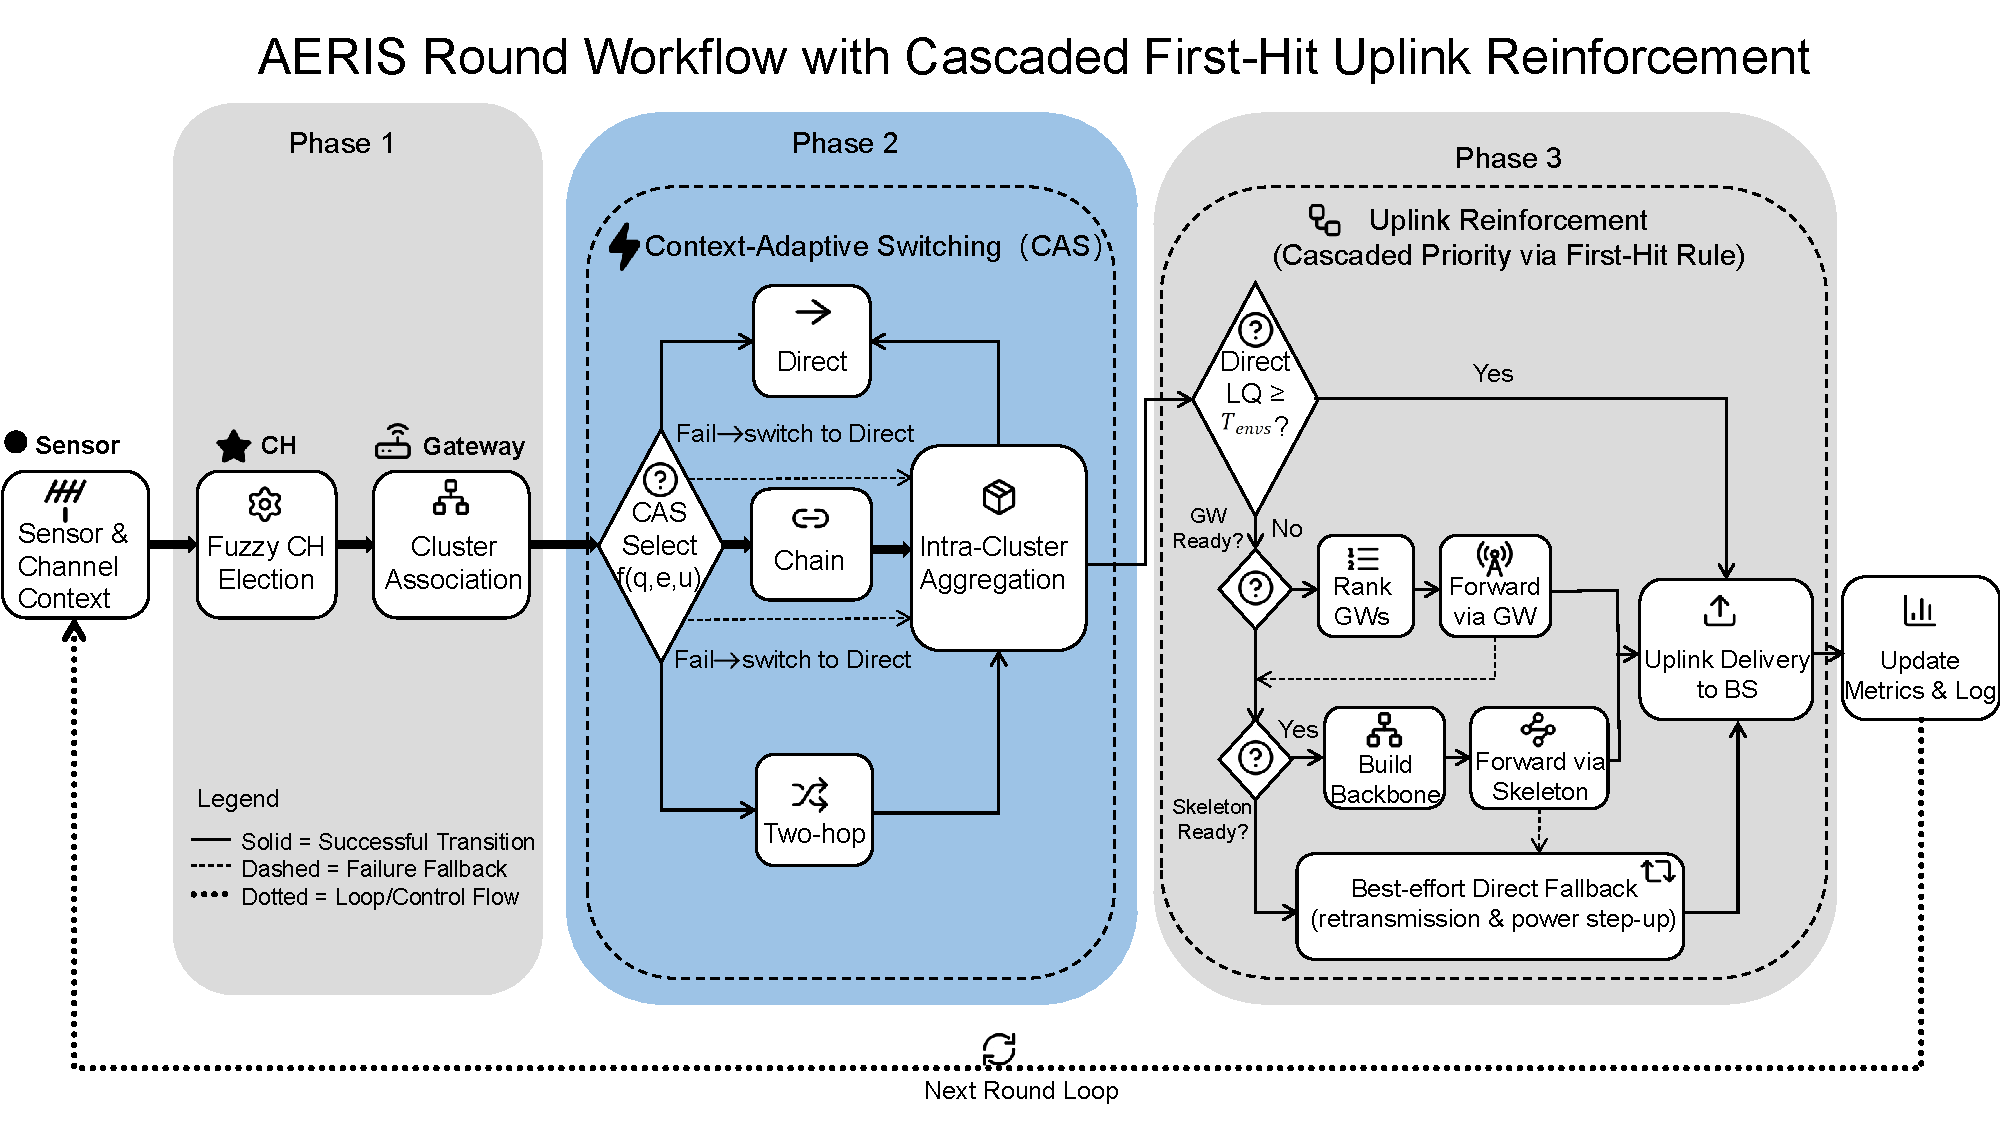
\includegraphics[width=0.90\textwidth]{fig0_aeris_workflow_temp_20260420.pdf}
\caption{AERIS round workflow with cascaded uplink reinforcement.}
\label{fig:aeris_workflow}
\end{figure*}

\section{Protocol Design}
AERIS combines CAS for intra-cluster transmission mode selection, Gateway reinforcement for cluster-head to base-station uplinks, and Skeleton forwarding for sparse CH fallback routes. The goal is to add reliability support only where direct forwarding becomes unreliable, while keeping online logic deterministic and auditable.

Gateway candidates are ranked by a fixed linear score,
\begin{equation}
\mathrm{Score}_i = \alpha \hat{E}_i + \beta \hat{C}_i + \gamma \hat{L}_i + \delta \hat{D}_i,
\end{equation}
where $\hat{E}_i$, $\hat{C}_i$, $\hat{L}_i$, and $\hat{D}_i$ denote normalized residual energy, centrality, link quality, and CH-to-BS distance. In this implementation, centrality is a distance-aware neighborhood surrogate computed from local geometry, link quality is the current channel-estimated success probability for the candidate hop, and all scalar features are normalized to $[0,1]$ before scoring. CAS uses another fixed linear rule over \{direct, chain, two-hop\}; the shared coefficients are held constant across environments in publication-tier runs, so mode selection is reproducible under identical inputs and seeds:
\begin{equation}
m^{\star}=\arg\max_{m \in \{\mathrm{direct},\mathrm{chain},\mathrm{two\mbox{-}hop}\}} \left( a_m \hat{q} + b_m \hat{e} + c_m \hat{u} \right),
\end{equation}
where $\hat{q}$, $\hat{e}$, and $\hat{u}$ are normalized local channel quality, residual energy, and utilization terms, and the coefficients $\{a_m,b_m,c_m\}$ are fixed for each candidate mode. Skeleton forwarding is built as a sparse CH relay backbone after clustering and is refreshed round-by-round together with the CH set; in the audited publication configuration it acts as a reserve fallback path rather than an actively exercised mechanism.

The forwarding logic is cascaded rather than multipath. A cluster head first checks direct uplink quality, then tries Gateway support if available, then Skeleton support if available, and finally makes one last direct attempt. In the strict-physics regime, this ``best-effort direct fallback'' is a single direct transmission attempt without protocol-level retransmission.

In practice, the protocol only activates extra forwarding structure after a direct path has become unattractive under the current channel estimate. CAS decides whether a sensor-to-CH transfer stays direct, switches to a short chain, or uses a two-hop relay; Gateway support then targets the more fragile CH-to-BS segment; Skeleton remains a reserve fallback if Gateway support is unavailable. The control path is deliberately narrow: AERIS does not search a large policy space online, and the same inputs always trigger the same routing decisions.

AERIS is an engineering design rather than a formal routing theorem. It adds alternate forwarding structure only when the direct path looks weak, reacts to a small number of local conditions with fixed rules, and is therefore judged by how that choice changes delivery and cost in deployment.

\subsection{Why the Modules Are Ordered This Way}
The ordering of the modules is part of the design rather than an implementation detail. Direct transmission is checked first because it is the cheapest option whenever the channel still supports it. Gateway support comes next because the audited experiments show that the CH-to-BS segment is usually the first place where reliability collapses in harsher cells. Skeleton forwarding is deliberately placed behind Gateway support because it is intended to preserve a fallback path, not to replace the main uplink rule.

This ordering also keeps the policy interpretable. AERIS does not ask every round whether all possible forwarding structures should be explored. Instead, it asks a smaller sequence of questions: is direct transmission still reasonable, is there a nearby Gateway that can protect the uplink, and if not, does the sparse Skeleton path exist? The protocol therefore behaves like a controlled escalation path rather than a broad route search.

\subsection{Intended Operating Regime}
The design is aimed at deployments where channel quality varies significantly across the field and where a modest increase in runtime complexity is acceptable if it stabilizes delivery. It is not aimed at the cleanest office-like regimes, where the longest-lived chain often remains the better choice, and it is not aimed at routing stacks that can afford heavier control traffic or training-time optimization. This intended operating regime is important in reading the evaluation, because it explains why the paper compares AERIS against classical baselines but interprets the result as deployment guidance rather than universal ranking.

\section{Evaluation Setup}
The primary metric is packet delivery ratio over expected application-layer transmissions,
\begin{equation}
\mathrm{PDR}_{\mathrm{expected}}=\frac{N_{\mathrm{delivered}}}{N_{\mathrm{expected}}},
\end{equation}
where $N_{\mathrm{expected}}$ counts one packet per alive source node per round even if a protocol suppresses actual transmission. This denominator is kept fixed across protocols so that the reliability comparison is not quietly changed by protocol-specific reporting logic.

We use complementary settings. The first is a five-protocol NS-3 audit against AERIS, LEACH, PEGASIS, HEED, and TEEN across four environments and 100, 500, and 1000 nodes ($n=30$ per environment-node-protocol cell). The second is an expanded dual-machine NS-3 boundary sweep that adds CTP and RPL-MRHOF and covers 50, 100, 200, 300, 500, 800, and 1000 nodes. In the standalone NS-3 harness, CTP and RPL-MRHOF are implemented as collection-tree baselines rather than complete LLN protocol stacks: CTP favors progress-constrained link-cost forwarding toward the sink, while RPL-MRHOF uses accumulated path cost for parent/path selection. We therefore interpret them as stronger collection-style baselines for boundary mapping, not as exhaustive replacements for full standards-compliant RPL, ORPL, ORW, or TSCH-based LLN stacks. The third is a 3360-run NS-3 AERIS ablation matrix over the same four environments and seven node counts, comparing full AERIS with no-Gateway, no-CAS, and no-CH-score variants. The fourth setting is a strict-physics Python simulator matrix across four environments and 100--1000 nodes ($n=3200$ per environment-node-protocol cell) with explicit collision and relay stress; in that layer, LEACH, HEED, and TEEN are reported in minimally adapted relay-enabled form for multi-hop comparability. To avoid relying on PDR alone, we also report total energy, lifetime, first-node death, and hop count in the frozen 100-node publication block. Mechanism and trade-off analysis use that block together with an audited 400-replicate AERIS mechanism matrix.

The four environments are used consistently across all experiments: indoor office, indoor factory, outdoor suburban, and outdoor urban. They are meant to cover a progression from relatively benign links to much harsher settings. The node counts then separate small-network behavior from the denser cells where poor CH-to-BS links and relay pressure become more visible.

This role split is deliberate. The five-protocol NS-3 audit asks whether AERIS beats the classical WSN baselines under one native simulation harness. The expanded seven-protocol sweep asks whether that result survives contact with stronger collection-tree baselines. The NS-3 ablation asks which AERIS module actually carries the delivery gain, while the strict-physics simulator tests the classical-baseline story under stronger relay and collision assumptions in an adapted stress layer rather than in a second canonical ranking layer. Lifetime, first-node death, hop count, and total energy then show whether delivery gains come from spreading or concentrating load. Keeping these layers separate prevents stress evidence from being mistaken for native baseline ranking.

\begin{table}[t]
\caption{Experimental settings used in the paper.}
\label{tbl:exp_settings}
\centering
\scriptsize
\setlength{\tabcolsep}{3pt}
\begin{tabular}{lcccc}
\toprule
Layer & Platform & Protocols & Cells & Role \\
\midrule
Classical audit & NS-3 & 5 protocols & $4 \times 3$ & anchor \\
Expanded audit & NS-3 & 7 protocols & $4 \times 7$ & boundary \\
Module ablation & NS-3 & 4 AERIS variants & $4 \times 7$ & attribution \\
Strict & Python & adapted 5-protocol & $4 \times 6$ & stress \\
Mechanism & Python & AERIS-only grid & $4 \times 3$ & attribution \\
Frozen block & pooled stats & 5-protocol summary & 100-node only & trade-off \\
\bottomrule
\end{tabular}
\end{table}
\section{Results}
\begin{figure*}[t]
\centering
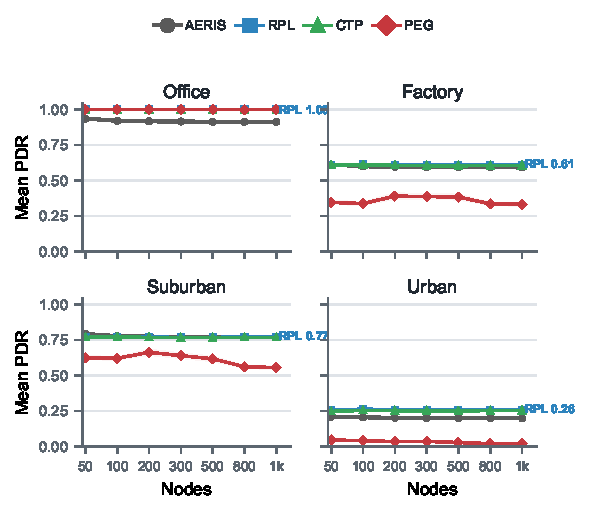
\includegraphics[width=0.98\textwidth]{fig_lcn26_ns3_expanded_boundary.pdf}
\caption{Expanded seven-protocol NS-3 boundary map across four environments and 50--1000 nodes ($n=30$ per cell). Panel (a) marks the mean-PDR winner in each cell, while very small absolute gaps should be interpreted as near-ties rather than strong superiority claims. Panel (b) gives AERIS's PDR gap to the cell winner in percentage points. Panels (c) and (d) show how AERIS's rank changes when the baseline family expands from classical WSN protocols to CTP/RPL-MRHOF collection baselines.}
\label{fig:ns3_boundary}
\end{figure*}

\subsection{Expanded NS-3 Boundary}
Figure~\ref{fig:ns3_boundary} gives the main boundary result from the seven-protocol dual-machine NS-3 sweep. If the baseline family is restricted to classical WSN protocols, AERIS is rank-1 in 21 of 28 environment-node cells and top-2 in all 28. This supports the classical-baseline claim: AERIS is a strong reliability-first design relative to LEACH, PEGASIS, HEED, and TEEN outside the benign office regime.

The expanded audit also shows why that claim must be bounded. Once CTP and RPL-MRHOF are included, AERIS remains strongest mainly in outdoor suburban cells: it wins 6 of 7 scales and is essentially tied at 1000 nodes, where RPL-MRHOF leads by only 0.0001 PDR points in the dual sweep. Such cells should be read as near-ties rather than practical superiority claims. In contrast, CTP leads the office cells, and RPL-MRHOF leads most factory and urban cells. AERIS is slightly ahead at factory-50, but falls 1.3--1.8 percentage points behind RPL-MRHOF at larger factory scales; in urban, the average gap to the winner is 5.69 points.

This boundary is the main practical outcome of the expanded audit. AERIS solves a weakness of the classical clustering/chain baselines by protecting fragile uplinks with Gateway support, but collection-tree and RPL-style baselines already solve part of that path-selection problem with richer parent choice. The strongest defensible claim is therefore not that AERIS is globally best, but that its rule-based control path delivers a large gain over classical WSN baselines and remains competitive or best in selected harsh-channel regimes, especially suburban cells.

\subsection{Classical Audit and Stress Evidence}
The five-protocol NS-3 audit remains useful as the classical-baseline anchor. In that subset, PEGASIS is best in indoor office, while AERIS leads in factory, suburban, and urban conditions. At 1000 nodes, AERIS reaches 0.593 in indoor factory, 0.770 in outdoor suburban, and 0.200 in outdoor urban, compared with 0.324, 0.549, and 0.019 for PEGASIS. This is why the expanded result should be read as a boundary refinement rather than a reversal of the classical-baseline claim.

The strict-physics matrix asks whether the classical-baseline ordering survives once collision and relay stress are made explicit in the adapted layer. Figure~\ref{fig:strict_python} shows that it does. PEGASIS remains strongest in indoor office (0.991 at 100 nodes and 0.988 at 1000), whereas AERIS stays rank-1 in indoor factory, outdoor suburban, and outdoor urban. At 1000 nodes, AERIS remains well above PEGASIS in indoor factory (0.728 vs. 0.300) and outdoor suburban (0.728 vs. 0.473), and it still leads in outdoor urban (0.136 vs. 0.099).

This matrix is not the main fairness anchor because LEACH, HEED, and TEEN are minimally augmented with a simple relay layer for multi-hop comparability in this setting. We therefore do not interpret Fig.~\ref{fig:strict_python} as a second canonical protocol ranking. Its role is narrower: to show that AERIS's harsh-channel advantage is not erased by explicit collision-and-relay stress even though absolute PDR falls for every protocol in the harder scales.

\begin{figure}[t]
\centering

\includegraphics[width=\columnwidth]{fig_lcn26_strict_compact.pdf}
\caption{Strict-physics Python adapted stress test across four environments and 100--1000 nodes ($n=3200$ per cell). LEACH, HEED, and TEEN appear here in minimally relay-enabled form for strict-layer comparability; this layer tests collision-and-relay stress and is not used as canonical ranking evidence.}
\label{fig:strict_python}
\end{figure}

\subsection{Ablation and Deployment Boundary}
Figure~\ref{fig:ablation} gives the expanded NS-3 module attribution test. It reruns full AERIS and three ablated variants over the four-environment, seven-scale matrix used in the boundary audit, for 3360 experiments in total. The result is sharper than the earlier frozen 100-node ablation: Gateway is the main gain carrier in factory and suburban cells. Removing Gateway costs 5.82 percentage points on average in factory and 7.58 points in suburban, with all seven node scales significant after Holm correction in both environments. It is essentially neutral in office and weak in urban, which is consistent with the boundary result: office does not need extra uplink protection, while urban links can become too poor for a nearby Gateway to rescue reliably.

\begin{figure*}[t]
\centering

\includegraphics[width=0.98\textwidth]{fig_lcn26_ns3_ablation_expanded.pdf}
\caption{Expanded NS-3 AERIS ablation across four environments and 50--1000 nodes ($n=30$ per cell). Heatmaps show the PDR contribution of each module, computed as full AERIS minus the ablated variant in percentage points; dots mark cells significant after Holm correction. Gateway carries the factory/suburban gain, CAS is environment-dependent, and CH-score removal is near-neutral in this audited configuration. Skeleton is treated as a reserve fallback rather than an observed dominant gain source.}
\label{fig:ablation}
\end{figure*}

CAS behaves differently. Removing CAS is beneficial in office and suburban cells, but hurts urban delivery by 0.91 points on average, with five of seven urban scales significant. This means CAS is not a universal gain module; it is useful mainly when a short local detour remains viable under harsh links. Removing the CH scoring component is near-neutral in all environments. This does not make the score irrelevant to the design, but it does show that the measured delivery gain in this publication configuration should not be attributed to head scoring.

The audited 400-replicate mechanism matrix is summarized in Fig.~\ref{fig:mechanism}. Gateway uplink PDR stays near 1.0 in office, factory, and suburban cells, but drops sharply at urban-1000, exactly where end-to-end PDR collapses. A targeted follow-up rerun of the three harsh 1000-node cells on FatMachine reproduced the same bottleneck pattern to the reported precision. The visual takeaway is the same as the ablation: Gateway carries the gain, CAS is conditional, and Skeleton remains dormant in the audited configuration.

\begin{figure}[t]
\centering

\includegraphics[width=\columnwidth]{fig_lcn26_mechanism_compact.pdf}
\caption{AERIS mechanism matrix from 400 audited replicates across 12 environment-node cells. The top panel shows end-to-end PDR and gateway uplink PDR; the lower panel shows first-node death and CAS two-hop share. Gateway remains near-perfect in office, factory, and suburban cells, but collapses at urban-1000; early FND exposes the reliability-lifetime cost of concentrated relay roles.}
\label{fig:mechanism}
\end{figure}

\begin{table}[t]
\caption{Frozen 100-node publication block pooled across protocols. AERIS has the highest pooled PDR and lowest total energy, but also the shortest lifetime and early FND, making the reliability-lifetime trade-off explicit.}
\label{tbl:pooled_summary}
\centering
\scriptsize
\setlength{\tabcolsep}{3pt}
\begin{tabular}{lccccc}
\toprule
Method & PDR$\uparrow$ & Energy$\downarrow$ & Lifetime$\uparrow$ & FND$\uparrow$ & Hops$\downarrow$ \\
\midrule
AERIS & 0.674 & 131.1 & 215.5 & 15.8 & 1.98 \\
PEGASIS & 0.373 & 137.6 & 300.0 & 70.7 & 32.37 \\
LEACH & 0.260 & 165.4 & 300.0 & 0.0 & 1.71 \\
HEED & 0.414 & 165.2 & 300.0 & 11.4 & 2.00 \\
TEEN & 0.432 & 159.4 & 299.0 & 0.0 & 1.28 \\
\bottomrule
\end{tabular}
\end{table}

The cost is just as clear. Table~\ref{tbl:pooled_summary} shows that AERIS has the lowest total energy (131.1 J) but the shortest lifetime (215.5 rounds). Fig.~\ref{fig:mechanism} shows where that cost appears inside the protocol: early node death and shrinking two-hop support in the harsh cells. Better delivery is bought with concentrated relay burden and rapid attrition once key forwarding roles are exhausted. This is the central engineering trade-off, not a secondary artifact of the evaluation.

Figures~\ref{fig:ns3_boundary}--\ref{fig:ablation} and Table~\ref{tbl:pooled_summary} suggest a more concrete deployment rule. If the target cell behaves more like the office regime, or if the design target is closer to the pooled long-lifetime profile of PEGASIS (300 rounds lifetime, 70.7-round FND) than to maximum delivery, PEGASIS or another simpler chain-based solution is the safer default among classical WSN protocols. If the deployment can use richer collection-tree or RPL-style path selection, CTP/RPL-MRHOF should also be considered first in office, factory, and urban regimes. AERIS is easiest to justify when the application needs a simple auditable WSN control path, the baseline family is closer to classical clustering/chain protocols, or the cell resembles the suburban regime where AERIS remains best or effectively tied even after CTP/RPL-MRHOF are added.

\subsection{When AERIS Should Not Be Chosen}
The office regime is the clearest negative case for AERIS. When direct, chain, or collection-tree forwarding is already highly reliable, the extra AERIS control structure does not buy enough to offset earlier node death. PEGASIS remains a credible classical deployment option in benign settings, and CTP/RPL-MRHOF are stronger still in the expanded NS-3 audit.

The same caution applies when the operating goal is longevity rather than delivery, or when the system already has a mature LLN stack available. AERIS can look attractive because its total energy is low, but the audited statistics show that it pays for delivery by exhausting key forwarding roles earlier. For applications that tolerate some delivery loss but require long unattended operation, that trade-off can make PEGASIS or another simpler chain-based design the better choice. For applications that can absorb RPL-style control structure, the expanded audit shows that RPL-MRHOF can dominate AERIS in factory and urban cells. In short: choose AERIS when delivery probability under harsh heterogeneous channels is the priority and a simple auditable controller is required; prefer PEGASIS-like routing for lifetime-first classical deployments; prefer CTP/RPL-style routing when richer collection-tree control is acceptable; avoid AERIS in benign office-like regimes where extra structure buys little.

\section{Discussion and Limitations}
The main message is simple. AERIS is strongest as a simple reliability-first alternative to classical WSN baselines, especially in the suburban harsh-channel regime; it is not the default choice for benign office-like regimes, lifetime-dominated deployments, or settings where collection-tree/RPL-style routing is available and acceptable. Its gain should be attributed mainly to Gateway-assisted uplinks, not to all modules equally. This narrower reading is more useful than a universal winner claim, because it tells the reader where the rule-based design should and should not be deployed.

Several limits remain. The expanded NS-3 audit includes CTP and RPL-MRHOF collection baselines, but not the full low-power routing space: opportunistic routing, ORPL/ORW-style candidate forwarding, coding-based reliability, channel hopping, and standards-compliant RPL stacks remain outside this evidence package. The strict-physics layer is deployment-stress evidence rather than external ground truth, and its MAC abstraction still omits full 802.15.4/TSCH/CSMA-CA behavior such as ACK loops, backoff dynamics, capture effects, and channel hopping. Recent LLN work likewise emphasizes scalable path management and control-plane flexibility as open problems \cite{almutairi2024survey,djennadi2025exploring}. Because TEEN is event-triggered, $\mathrm{PDR}_{\mathrm{expected}}$ should be read together with energy, lifetime, FND, and hop count. The current study is also limited to static topologies, the tested environment taxonomy, and artifacts that are not yet public.

The provenance chain is intentionally explicit. The five-protocol NS-3 rerun anchors the classical-baseline comparison, the seven-protocol dual-machine sweep maps the CTP/RPL-MRHOF boundary, the strict-physics layer stress-tests the classical-baseline story, the AERIS-only mechanism grid attributes the gain to Gateway support and selected two-hop use, and the pooled 100-node block keeps energy, lifetime, FND, and hops visible. A separate FatMachine rerun of the three harsh 1000-node mechanism cells reproduced the key bottleneck means to the reported precision. This separation keeps independent-platform evidence distinct from stress evidence.

\section{Conclusion}
This paper revisited AERIS as a reliable WSN routing design and reevaluated it with a five-protocol NS-3 audit, an expanded seven-protocol CTP/RPL-MRHOF boundary sweep, a strict-physics simulator matrix, and audited mechanism evidence. The resulting claim is deliberately bounded: AERIS is a strong reliability-first alternative to classical WSN baselines, with gains carried mainly by Gateway support, but richer collection-tree routing narrows or removes that advantage in office, factory, and urban regimes. It also buys delivery by concentrating forwarding work, which shortens lifetime and advances first-node death. The practical contribution is therefore a visible deployment boundary rather than a global leaderboard.

Future work should compare against full RPL/ORPL/ORW-style stacks, add more realistic MAC behavior, and test whether Gateway-style reinforcement can be combined with collection-tree parent selection without reproducing the early-node-death cost.

\FloatBarrier
\balance
\bibliographystyle{IEEEtran}
\bibliography{ref}

\end{document}
